\PassOptionsToPackage{unicode=true}{hyperref} % options for packages loaded elsewhere
\PassOptionsToPackage{hyphens}{url}
%
\documentclass[]{book}
\usepackage{lmodern}
\usepackage{amssymb,amsmath}
\usepackage{ifxetex,ifluatex}
\usepackage{fixltx2e} % provides \textsubscript
\ifnum 0\ifxetex 1\fi\ifluatex 1\fi=0 % if pdftex
  \usepackage[T1]{fontenc}
  \usepackage[utf8]{inputenc}
  \usepackage{textcomp} % provides euro and other symbols
\else % if luatex or xelatex
  \usepackage{unicode-math}
  \defaultfontfeatures{Ligatures=TeX,Scale=MatchLowercase}
\fi
% use upquote if available, for straight quotes in verbatim environments
\IfFileExists{upquote.sty}{\usepackage{upquote}}{}
% use microtype if available
\IfFileExists{microtype.sty}{%
\usepackage[]{microtype}
\UseMicrotypeSet[protrusion]{basicmath} % disable protrusion for tt fonts
}{}
\IfFileExists{parskip.sty}{%
\usepackage{parskip}
}{% else
\setlength{\parindent}{0pt}
\setlength{\parskip}{6pt plus 2pt minus 1pt}
}
\usepackage{hyperref}
\hypersetup{
            pdftitle={Standardizing-Marine-Biological-Data},
            pdfauthor={Brett Johnson},
            pdfborder={0 0 0},
            breaklinks=true}
\urlstyle{same}  % don't use monospace font for urls
\usepackage{color}
\usepackage{fancyvrb}
\newcommand{\VerbBar}{|}
\newcommand{\VERB}{\Verb[commandchars=\\\{\}]}
\DefineVerbatimEnvironment{Highlighting}{Verbatim}{commandchars=\\\{\}}
% Add ',fontsize=\small' for more characters per line
\usepackage{framed}
\definecolor{shadecolor}{RGB}{248,248,248}
\newenvironment{Shaded}{\begin{snugshade}}{\end{snugshade}}
\newcommand{\AlertTok}[1]{\textcolor[rgb]{0.94,0.16,0.16}{#1}}
\newcommand{\AnnotationTok}[1]{\textcolor[rgb]{0.56,0.35,0.01}{\textbf{\textit{#1}}}}
\newcommand{\AttributeTok}[1]{\textcolor[rgb]{0.77,0.63,0.00}{#1}}
\newcommand{\BaseNTok}[1]{\textcolor[rgb]{0.00,0.00,0.81}{#1}}
\newcommand{\BuiltInTok}[1]{#1}
\newcommand{\CharTok}[1]{\textcolor[rgb]{0.31,0.60,0.02}{#1}}
\newcommand{\CommentTok}[1]{\textcolor[rgb]{0.56,0.35,0.01}{\textit{#1}}}
\newcommand{\CommentVarTok}[1]{\textcolor[rgb]{0.56,0.35,0.01}{\textbf{\textit{#1}}}}
\newcommand{\ConstantTok}[1]{\textcolor[rgb]{0.00,0.00,0.00}{#1}}
\newcommand{\ControlFlowTok}[1]{\textcolor[rgb]{0.13,0.29,0.53}{\textbf{#1}}}
\newcommand{\DataTypeTok}[1]{\textcolor[rgb]{0.13,0.29,0.53}{#1}}
\newcommand{\DecValTok}[1]{\textcolor[rgb]{0.00,0.00,0.81}{#1}}
\newcommand{\DocumentationTok}[1]{\textcolor[rgb]{0.56,0.35,0.01}{\textbf{\textit{#1}}}}
\newcommand{\ErrorTok}[1]{\textcolor[rgb]{0.64,0.00,0.00}{\textbf{#1}}}
\newcommand{\ExtensionTok}[1]{#1}
\newcommand{\FloatTok}[1]{\textcolor[rgb]{0.00,0.00,0.81}{#1}}
\newcommand{\FunctionTok}[1]{\textcolor[rgb]{0.00,0.00,0.00}{#1}}
\newcommand{\ImportTok}[1]{#1}
\newcommand{\InformationTok}[1]{\textcolor[rgb]{0.56,0.35,0.01}{\textbf{\textit{#1}}}}
\newcommand{\KeywordTok}[1]{\textcolor[rgb]{0.13,0.29,0.53}{\textbf{#1}}}
\newcommand{\NormalTok}[1]{#1}
\newcommand{\OperatorTok}[1]{\textcolor[rgb]{0.81,0.36,0.00}{\textbf{#1}}}
\newcommand{\OtherTok}[1]{\textcolor[rgb]{0.56,0.35,0.01}{#1}}
\newcommand{\PreprocessorTok}[1]{\textcolor[rgb]{0.56,0.35,0.01}{\textit{#1}}}
\newcommand{\RegionMarkerTok}[1]{#1}
\newcommand{\SpecialCharTok}[1]{\textcolor[rgb]{0.00,0.00,0.00}{#1}}
\newcommand{\SpecialStringTok}[1]{\textcolor[rgb]{0.31,0.60,0.02}{#1}}
\newcommand{\StringTok}[1]{\textcolor[rgb]{0.31,0.60,0.02}{#1}}
\newcommand{\VariableTok}[1]{\textcolor[rgb]{0.00,0.00,0.00}{#1}}
\newcommand{\VerbatimStringTok}[1]{\textcolor[rgb]{0.31,0.60,0.02}{#1}}
\newcommand{\WarningTok}[1]{\textcolor[rgb]{0.56,0.35,0.01}{\textbf{\textit{#1}}}}
\usepackage{longtable,booktabs}
% Fix footnotes in tables (requires footnote package)
\IfFileExists{footnote.sty}{\usepackage{footnote}\makesavenoteenv{longtable}}{}
\usepackage{graphicx,grffile}
\makeatletter
\def\maxwidth{\ifdim\Gin@nat@width>\linewidth\linewidth\else\Gin@nat@width\fi}
\def\maxheight{\ifdim\Gin@nat@height>\textheight\textheight\else\Gin@nat@height\fi}
\makeatother
% Scale images if necessary, so that they will not overflow the page
% margins by default, and it is still possible to overwrite the defaults
% using explicit options in \includegraphics[width, height, ...]{}
\setkeys{Gin}{width=\maxwidth,height=\maxheight,keepaspectratio}
\setlength{\emergencystretch}{3em}  % prevent overfull lines
\providecommand{\tightlist}{%
  \setlength{\itemsep}{0pt}\setlength{\parskip}{0pt}}
\setcounter{secnumdepth}{5}
% Redefines (sub)paragraphs to behave more like sections
\ifx\paragraph\undefined\else
\let\oldparagraph\paragraph
\renewcommand{\paragraph}[1]{\oldparagraph{#1}\mbox{}}
\fi
\ifx\subparagraph\undefined\else
\let\oldsubparagraph\subparagraph
\renewcommand{\subparagraph}[1]{\oldsubparagraph{#1}\mbox{}}
\fi

% set default figure placement to htbp
\makeatletter
\def\fps@figure{htbp}
\makeatother

\usepackage{booktabs}
\usepackage[]{natbib}
\bibliographystyle{apalike}

\title{Standardizing-Marine-Biological-Data}
\author{Brett Johnson}
\date{2020-08-20}

\begin{document}
\maketitle

{
\setcounter{tocdepth}{1}
\tableofcontents
}
Biological data structures, definitions, measurements, and linkages are neccessarily as diverse as the systems they represent. This presents a real challenge when integrating data across biological research domains such as ecology, oceanography, fisheries, and climate sciences.

\hypertarget{intro}{%
\chapter{Introduction}\label{intro}}

The world of standardizing marine biological data is complex and fraught with uncertainty for naive oceanographer, biologist, scientist, or programmer.
This is about stacking the right standards for your desired interoperability with other data types.
For example, interoperating fish biology measurements with climate level variables.
There are a few links neccessary to make this possible and will permit broader access to better ecosystem based models.
This phenomena is not unique to specic scientific domains, but is rather pervasive as many scientific domains are currently being reshaped in light of recent advances in computing power, technology, and data science.

\hypertarget{data-structures}{%
\section{Data Structures}\label{data-structures}}

The OBIS-ENV Darwin Core Archive Data Structure.

\href{\%22https://obis.org/manual/\%22}{OBIS manual}

\hypertarget{ontologies-controlled-vocabularies}{%
\section{Ontologies \& Controlled Vocabularies}\label{ontologies-controlled-vocabularies}}

An ontology is a classification system for establishing a hierarchically related set of concepts. Concepts are often terms from controlled vocabularies.

From Marine Metadata: \# TODO: add link

"Ontologies can include all of the following, but are not required to include them, depending on which perspective from above you adhere to:

Classes (general things, types of things)
Instances (individual things)
Relationships among things
Properties of things
Functions, processes, constraints, and rules relating to things"

TODO: Research Unified Modeling Language?

There are a number of controlled vocabularies that are used to describe parameters commonly used in specific research domains. This allows for greater interoperability of data sets within the domain, and ideally between domains. Here, we strive to document a number of relevant examples.

\begin{itemize}
\item
  \href{\%22http://cfconventions.org/standard-names.html\%22}{Climate and Format (CF) Standard Names} are applied to sensors for application with OPeNDAP web service.
\item
  \href{\%22http://vocab.nerc.ac.uk/collection/L05/current/\%22}{Device categories} using the SeaDataNet device categories in NERC 2.0
\item
  \href{\%22http://vocab.nerc.ac.uk/collection/L22/current/\%22}{Device make/model using the SeaVoX Device Catalogue} in NERC 2.0,
\item
  \href{\%22http://vocab.nerc.ac.uk/collection/L06/current/\%22}{Platform categories using SeaVoX Platform Categories} in NERC 2.0
\item
  \href{\%22http://vocab.nerc.ac.uk/collection/C17/current/\%22}{Platform instances using the ICES Platform Codes} in NERC 2.0
\item
  \href{\%22http://vocab.nerc.ac.uk/collection/P06/current/\%22}{Unit of measure}
\item
  \href{\%22http://vocab.nerc.ac.uk/collection/P04/current/\%22}{GCMD Keywords (NASA)}
\item
  \href{\%22http://vocab.nerc.ac.uk/collection/C19/current/\%22}{Geographic Domain/Features of Interest}
\item
  \href{http://schema.geolink.org/1.0/base/main.html}{GeoLink base ontology} was part of the \href{http://www.geolink.org/}{EarthCube GeoLink Project}
\end{itemize}

TODO: Improve this paragraph
There are numberous ways to investigate which controlled vocabulary to use and this can be fairly overwhelming. For a simplified overview see \href{\%22http://seadatanet.maris2.nl/v_bodc_vocab_v2/vocab_relations.asp?lib=P08\%22}{here}.

Note: To describe a measurement or fact of a biological specimen that conforms to Darwin Core standards, it's neccessary to use the `Biological entity described elsewhere' method rather than taxon specific.

\hypertarget{collections}{%
\subsection{Collections}\label{collections}}

\hypertarget{oceanography}{%
\subsection{Oceanography}\label{oceanography}}

\href{http://www.bco-dmo.org/}{Biological and Chemcial Oceanography Data Management Office}

\href{https://mmisw.org/ont/\#/}{Marine metadata interoperability vocab resources}

\hypertarget{biology}{%
\subsection{Biology}\label{biology}}

\href{http://bioportal.bioontology.org/ontologies/ECSO}{BioPortal Ecosystem Ontology}

\hypertarget{nerc-search-interfaces}{%
\subsection{NERC Search Interfaces}\label{nerc-search-interfaces}}

\begin{itemize}
\item
  \href{http://seadatanet.maris2.nl/v_bodc_vocab_v2/welcome.asp}{SeaDatanet Common Vocab Search Interface:}
\item
  \href{https://www.seadatanet.org/Standards/Common-Vocabularies/}{SeaDataNet Common Vocabularies:}
\item
  \href{http://seadatanet.maris2.nl/v_bodc_vocab_v2/vocab_relations.asp?lib=P08}{SeaDataNet Vocab Library}
\end{itemize}

\hypertarget{geosciences}{%
\subsection{Geosciences}\label{geosciences}}

\href{https://www.unidata.ucar.edu/software/udunits/}{UDUNITS}are more common unit measurements in geosciences

\hypertarget{ecoenvo}{%
\subsection{Eco/EnvO}\label{ecoenvo}}

\href{\%22http://www.obofoundry.org/ontology/envo.html\%22}{Environment Ontology} including genomics.

\hypertarget{wild-cards}{%
\subsection{Wild Cards}\label{wild-cards}}

Question: Not sure use case for this.

\href{\%22https://www.bodc.ac.uk/resources/vocabularies/vocabulary_builder/biomodel/\%22}{P01 Biological Entity Parameter Code Builder}

\hypertarget{technologies}{%
\section{Technologies}\label{technologies}}

\hypertarget{erddap}{%
\subsection{ERDDAP}\label{erddap}}

\href{\%22https://coastwatch.pfeg.noaa.gov/erddap/index.html\%22}{ERDDAP} can be thought of as a data server. It provides `easier access to scientific data' by providing a consistent interface that aggregates many disparate data sources. It does this by providing translation services between many common file types for gridded arrarys (`net CDF' files) and tabular data (spreadsheets). Data access is also made easier because it unifies different types of data servers and access protocols. \href{\%22https://github.com/HakaiInstitute/erddap-basic\%22}{Here} is a basic erddap installation that walks you through how to load a data set.

\hypertarget{notes-on-integrating-obis-darwin-core-as-it-relates-to-ooss}{%
\section{Notes on Integrating OBIS, Darwin Core as it relates to OOS's}\label{notes-on-integrating-obis-darwin-core-as-it-relates-to-ooss}}

\hypertarget{metadata}{%
\section{Metadata}\label{metadata}}

OBIS uses the \href{http://rs.gbif.org/schema/eml-gbif-profile/1.1/eml-gbif-profile.xsd}{GBIF EML profile} (version 1.1). In case data providers use ISO19115/ISO19139, there is a mapping available here: \url{http://rs.gbif.org/schema/eml-gbif-profile/1.1/eml2iso19139.xsl} This will be important for integrating OBIS datasets to OOS metadata profiles.

\hypertarget{data-qc}{%
\section{Data QC}\label{data-qc}}

There are a number of tools available to check the quality of data or check your data format against the expected standard.

\href{https://obis.org/manual/processing/}{OBIS Datatools} shows some great R packages for this.

\hypertarget{compliance-checking}{%
\subsection{Compliance Checking}\label{compliance-checking}}

LifeWatch Belgium provides a number of tools to check your data against.
Specifically you can test OBIS data format and see a map of your sample locations to check if they are on land.
See \url{http://www.lifewatch.be/data-services/}

\hypertarget{semantic-web-and-darwin-core}{%
\subsection{Semantic Web and Darwin Core}\label{semantic-web-and-darwin-core}}

\href{\%22http://www.semantic-web-journal.net/system/files/swj1093.pdf\%22}{Lessons learned from adapting the Darwin Core vocabulary standard for use in RDF}

\hypertarget{resource-description-framework}{%
\subsection{Resource Description Framework}\label{resource-description-framework}}

\href{\%22https://dwc.tdwg.org/rdf/\%22}{Darwin Core Resource Description Framework Guide}

\hypertarget{methods}{%
\chapter{Methods}\label{methods}}

We describe our methods in this chapter.

\hypertarget{applications}{%
\chapter{Applications}\label{applications}}

Some \emph{significant} applications are demonstrated in this chapter.

\hypertarget{salmon-ocean-ecology-data}{%
\section{Salmon Ocean Ecology Data}\label{salmon-ocean-ecology-data}}

One of the goals of the Hakai Institute and the Canadian Integrated Ocean Observing System (CIOOS) is to facilitate Open Science and FAIR (findable, accessible, interoperable, reusable) ecological and oceanographic data. In a concerted effort to adopt or establish how best to do that, several Hakai and CIOOS staff attended an International Ocean Observing System (IOOS) Code Sprint in Ann Arbour, Michigan between October 7--11, 2019, to discuss how to implement FAIR data principles for biological data collected in the marine environment.

The \href{https://dwc.tdwg.org}{Darwin Core} is a highly structured data format that standardizes data table relations, vocabularies, and defines field names. The Darwin Core defines three table types: \texttt{event}, \texttt{occurrence}, and \texttt{measurementOrFact}. This intuitively captures the way most ecologists conduct their research. Typically, a survey (event) is conducted and measurements, counts, or observations (collectively measurementOrFacts) are made regarding a specific habitat or species (occurrence).

In the following script I demonstrate how I go about converting a subset of the data collected from the Hakai Institute Juvenile Salmon Program and discuss challenges, solutions, pros and cons, and when and what's worthwhile to convert to Darwin Core.

The conversion of a dataset to Darwin Core is much easier if your data are already tidy (normalized) in which you represent your data in separate tables that reflect the hierarchical and related nature of your observations. If your data are not already in a consistent and structured format, the conversion would likely be very arduous and not intuitive.

\hypertarget{event}{%
\subsection{event}\label{event}}

The first step is to consider what you will define as an event in your data set. I defined the capture of fish using a purse seine net as the \texttt{event}. Therefore, each row in the \texttt{event} table is one deployment of a seine net and is assigned a unique \texttt{eventID}.

My process for conversion was to make a new table called \texttt{event} and map the standard Darwin Core column names to pre-existing columns that serve the same purpose in my original \texttt{seine\_data} table and populate the other required fields.

\begin{Shaded}
\begin{Highlighting}[]
\NormalTok{event <-}\StringTok{ }\KeywordTok{tibble}\NormalTok{(}\DataTypeTok{eventID =}\NormalTok{ survey_seines}\OperatorTok{$}\NormalTok{seine_id,}
                \DataTypeTok{eventDate =} \KeywordTok{date}\NormalTok{(survey_seines}\OperatorTok{$}\NormalTok{survey_date),}
                \DataTypeTok{decimalLatitude =}\NormalTok{ survey_seines}\OperatorTok{$}\NormalTok{lat,}
                \DataTypeTok{decimalLongitude =}\NormalTok{ survey_seines}\OperatorTok{$}\NormalTok{long,}
                \DataTypeTok{geodeticDatum =} \StringTok{"EPSG:4326 WGS84"}\NormalTok{,}
                \DataTypeTok{minimumDepthInMeters =} \DecValTok{0}\NormalTok{,}
                \DataTypeTok{maximumDepthInMeters =} \DecValTok{9}\NormalTok{, }\CommentTok{# seine depth is 9 m}
                \DataTypeTok{samplingProtocol =} \StringTok{"http://dx.doi.org/10.21966/1.566666"} \CommentTok{# This is the DOI for the Hakai Salmon Data Package that contains the smnpling protocol, as well as the complete data package}
\NormalTok{               ) }

\KeywordTok{write_csv}\NormalTok{(event, here}\OperatorTok{::}\KeywordTok{here}\NormalTok{(}\StringTok{"datasets"}\NormalTok{, }\StringTok{"hakai_salmon_data"}\NormalTok{, }\StringTok{"event.csv"}\NormalTok{))}
\end{Highlighting}
\end{Shaded}

\hypertarget{occurrence}{%
\subsection{occurrence}\label{occurrence}}

Next you'll want to determine what constitutes an occurrence for your data set. Because each event captures fish, I consider each fish to be an occurrence. Therefore, the unit of observation (each row) in the occurrence table is a fish. To link each occurrence to an event you need to include the \texttt{eventID} column for every occurrence so that you know what seine (event) each fish (occurrence) came from. You must also provide a globally unique identifier for each occurrence. I already have a locally unique identifier for each fish in the original \texttt{fish\_data} table called \texttt{ufn}. To make it globally unique I pre-pend the organization and research program metadata to the \texttt{ufn} column.

\begin{Shaded}
\begin{Highlighting}[]
\CommentTok{#TODO: Include bycatch data as well}

\CommentTok{## make table long first}
\NormalTok{seines_total_long <-}\StringTok{ }\NormalTok{survey_seines }\OperatorTok\StringTok{ }
\StringTok{  }\KeywordTok{select}\NormalTok{(seine_id, so_total, pi_total, cu_total, co_total, he_total, ck_total) }\OperatorTok\StringTok{ }
\StringTok{  }\KeywordTok{pivot_longer}\NormalTok{(}\OperatorTok{-}\NormalTok{seine_id, }\DataTypeTok{names_to =} \StringTok{"scientificName"}\NormalTok{, }\DataTypeTok{values_to =} \StringTok{"n"}\NormalTok{)}

\NormalTok{seines_total_long}\OperatorTok{$}\NormalTok{scientificName <-}\StringTok{ }\KeywordTok{recode}\NormalTok{(seines_total_long}\OperatorTok{$}\NormalTok{scientificName, }\DataTypeTok{so_total =} \StringTok{"Oncorhynchus nerka"}\NormalTok{, }\DataTypeTok{pi_total =} \StringTok{"Oncorhynchus gorbushca"}\NormalTok{, }\DataTypeTok{cu_total =} \StringTok{"Oncorhynchus keta"}\NormalTok{, }\DataTypeTok{co_total =} \StringTok{"Oncorhynchus kisutch"}\NormalTok{, }\DataTypeTok{ck_total =} \StringTok{"Oncorhynchus tshawytscha"}\NormalTok{, }\DataTypeTok{he_total =} \StringTok{"Clupea pallasii"}\NormalTok{) }

\NormalTok{seines_taken_long <-}\StringTok{ }\NormalTok{survey_seines }\OperatorTok
\StringTok{  }\KeywordTok{select}\NormalTok{(seine_id, so_taken, pi_taken, cu_taken, co_taken, he_taken, ck_taken) }\OperatorTok\StringTok{ }
\StringTok{  }\KeywordTok{pivot_longer}\NormalTok{(}\OperatorTok{-}\NormalTok{seine_id, }\DataTypeTok{names_to =} \StringTok{"scientificName"}\NormalTok{, }\DataTypeTok{values_to =} \StringTok{"n_taken"}\NormalTok{) }

\NormalTok{seines_taken_long}\OperatorTok{$}\NormalTok{scientificName <-}\StringTok{ }\KeywordTok{recode}\NormalTok{(seines_taken_long}\OperatorTok{$}\NormalTok{scientificName, }\DataTypeTok{so_taken =} \StringTok{"Oncorhynchus nerka"}\NormalTok{, }\DataTypeTok{pi_taken =} \StringTok{"Oncorhynchus gorbushca"}\NormalTok{, }\DataTypeTok{cu_taken =} \StringTok{"Oncorhynchus keta"}\NormalTok{, }\DataTypeTok{co_taken =} \StringTok{"Oncorhynchus kisutch"}\NormalTok{, }\DataTypeTok{ck_taken =} \StringTok{"Oncorhynchus tshawytscha"}\NormalTok{, }\DataTypeTok{he_taken =} \StringTok{"Clupea pallasii"}\NormalTok{) }

\CommentTok{## remove records that have already been assigned an ID  }
\NormalTok{seines_long <-}\StringTok{  }\KeywordTok{full_join}\NormalTok{(seines_total_long, seines_taken_long, }\DataTypeTok{by =} \KeywordTok{c}\NormalTok{(}\StringTok{"seine_id"}\NormalTok{, }\StringTok{"scientificName"}\NormalTok{)) }\OperatorTok\StringTok{ }
\StringTok{  }\KeywordTok{drop_na}\NormalTok{() }\OperatorTok\StringTok{ }
\StringTok{  }\KeywordTok{mutate}\NormalTok{(}\DataTypeTok{n_not_taken =}\NormalTok{ n }\OperatorTok{-}\StringTok{ }\NormalTok{n_taken) }\OperatorTok\StringTok{ }\CommentTok{#so_total includes the number taken so I subtract n_taken to get n_not_taken}
\StringTok{  }\KeywordTok{select}\NormalTok{(}\OperatorTok{-}\NormalTok{n_taken, }\OperatorTok{-}\NormalTok{n) }\OperatorTok\StringTok{ }
\StringTok{  }\KeywordTok{filter}\NormalTok{(n_not_taken }\OperatorTok{>}\StringTok{ }\DecValTok{0}\NormalTok{)}

\NormalTok{all_fish_caught <-}
\StringTok{  }\NormalTok{seines_long[}\KeywordTok{rep}\NormalTok{(}\KeywordTok{seq.int}\NormalTok{(}\DecValTok{1}\NormalTok{, }\KeywordTok{nrow}\NormalTok{(seines_long)), seines_long}\OperatorTok{$}\NormalTok{n_not_taken), }\DecValTok{1}\OperatorTok{:}\DecValTok{3}\NormalTok{] }\OperatorTok\StringTok{ }
\StringTok{  }\KeywordTok{select}\NormalTok{(}\OperatorTok{-}\NormalTok{n_not_taken) }\OperatorTok\StringTok{ }
\StringTok{  }\KeywordTok{mutate}\NormalTok{(}\DataTypeTok{prefix =} \StringTok{"hakai-jsp-"}\NormalTok{,}
         \DataTypeTok{suffix =} \DecValTok{1}\OperatorTok{:}\KeywordTok{nrow}\NormalTok{(.),}
         \DataTypeTok{occurrenceID =} \KeywordTok{paste0}\NormalTok{(prefix, suffix)}
\NormalTok{  ) }\OperatorTok\StringTok{ }
\StringTok{  }\KeywordTok{select}\NormalTok{(}\OperatorTok{-}\NormalTok{prefix, }\OperatorTok{-}\NormalTok{suffix)}

\CommentTok{#}

\CommentTok{# Change species names to full Scientific names }
\NormalTok{latin <-}\StringTok{ }\KeywordTok{fct_recode}\NormalTok{(fish_data}\OperatorTok{$}\NormalTok{species, }\StringTok{"Oncorhynchus nerka"}\NormalTok{ =}\StringTok{ "SO"}\NormalTok{, }\StringTok{"Oncorhynchus gorbuscha"}\NormalTok{ =}\StringTok{ "PI"}\NormalTok{, }\StringTok{"Oncorhynchus keta"}\NormalTok{ =}\StringTok{ "CU"}\NormalTok{, }\StringTok{"Oncorhynchus kisutch"}\NormalTok{ =}\StringTok{ "CO"}\NormalTok{, }\StringTok{"Clupea pallasii"}\NormalTok{ =}\StringTok{ "HE"}\NormalTok{, }\StringTok{"Oncorhynchus tshawytscha"}\NormalTok{ =}\StringTok{ "CK"}\NormalTok{) }\OperatorTok\StringTok{ }
\StringTok{  }\KeywordTok{as.character}\NormalTok{()}

\NormalTok{fish_retained_data <-}\StringTok{ }\NormalTok{fish_data }\OperatorTok\StringTok{ }
\StringTok{  }\KeywordTok{mutate}\NormalTok{(}\DataTypeTok{scientificName =}\NormalTok{ latin) }\OperatorTok\StringTok{ }
\StringTok{  }\KeywordTok{select}\NormalTok{(}\OperatorTok{-}\NormalTok{species) }\OperatorTok\StringTok{ }
\StringTok{  }\KeywordTok{mutate}\NormalTok{(}\DataTypeTok{prefix =} \StringTok{"hakai-jsp-"}\NormalTok{,}
         \DataTypeTok{occurrenceID =} \KeywordTok{paste0}\NormalTok{(prefix, ufn)) }\OperatorTok\StringTok{ }
\StringTok{  }\KeywordTok{select}\NormalTok{(}\OperatorTok{-}\NormalTok{semsp_id, }\OperatorTok{-}\NormalTok{prefix, }\OperatorTok{-}\NormalTok{ufn, }\OperatorTok{-}\NormalTok{fork_length_field, }\OperatorTok{-}\NormalTok{fork_length, }\OperatorTok{-}\NormalTok{weight, }\OperatorTok{-}\NormalTok{weight_field)}

\NormalTok{occurrence <-}\StringTok{ }\KeywordTok{bind_rows}\NormalTok{(all_fish_caught, fish_retained_data) }\OperatorTok\StringTok{ }
\StringTok{  }\KeywordTok{mutate}\NormalTok{(}\DataTypeTok{basisOfRecord =} \StringTok{"HumanObservation"}\NormalTok{,}
        \DataTypeTok{occurenceStatus =} \StringTok{"present"}\NormalTok{) }\OperatorTok\StringTok{ }
\StringTok{  }\KeywordTok{rename}\NormalTok{(}\DataTypeTok{eventID =}\NormalTok{ seine_id)}
\end{Highlighting}
\end{Shaded}

For each occurrence of the six different fish species that I caught I need to match the species name that I provide with the official \texttt{scientificName} that is part of the World Register of Marine Species database \url{http://www.marinespecies.org/}

\begin{Shaded}
\begin{Highlighting}[]
\CommentTok{# I went directly to the WoRMS webite (http://www.marinespecies.org/) to download the full taxonomic levels for the salmon species I have and put the WoRMS output (species_matched.xls) table in this project directory which is read in below and joined with the occurrence table}

\NormalTok{species_matched <-}\StringTok{ }\NormalTok{readxl}\OperatorTok{::}\KeywordTok{read_excel}\NormalTok{(here}\OperatorTok{::}\KeywordTok{here}\NormalTok{(}\StringTok{"datasets"}\NormalTok{, }\StringTok{"hakai_salmon_data"}\NormalTok{, }\StringTok{"raw_data"}\NormalTok{, }\StringTok{"species_matched.xls"}\NormalTok{))}

\NormalTok{occurrence <-}\StringTok{ }\KeywordTok{left_join}\NormalTok{(occurrence, species_matched, }\DataTypeTok{by =} \KeywordTok{c}\NormalTok{(}\StringTok{"scientificName"}\NormalTok{ =}\StringTok{ "ScientificName"}\NormalTok{)) }\OperatorTok\StringTok{ }
\StringTok{  }\KeywordTok{select}\NormalTok{(occurrenceID, basisOfRecord, scientificName, eventID, }\DataTypeTok{occurrenceStatus =}\NormalTok{ occurenceStatus, Kingdom, Phylum, Class, Order, Family, Genus, Species)}

\KeywordTok{write_csv}\NormalTok{(occurrence, here}\OperatorTok{::}\KeywordTok{here}\NormalTok{(}\StringTok{"datasets"}\NormalTok{, }\StringTok{"hakai_salmon_data"}\NormalTok{, }\StringTok{"occurrence.csv"}\NormalTok{))}
\end{Highlighting}
\end{Shaded}

\hypertarget{measurementorfact}{%
\subsection{measurementOrFact}\label{measurementorfact}}

To convert all your measurements or facts from your normal format to Darwin Core you essentially need to put all your measurements into one column called measurementType and a corresponding column called measurementValue. This standardizes the column names are in the \texttt{measurementOrFact} table. There are a number of predefined \texttt{measurementType}s listed on the \href{https://www.bodc.ac.uk/resources/vocabularies/}{NERC} database that should be used where possible. I found it difficult to navigate this page to find the correct \texttt{measurementType}.

Here I convert length, and weight measurements that relate to an event and an occurrence and call those \texttt{measurementTypes} as \texttt{length} and \texttt{weight}.

\begin{Shaded}
\begin{Highlighting}[]
\NormalTok{fish_data}\OperatorTok{$}\NormalTok{weight <-}\StringTok{ }\KeywordTok{coalesce}\NormalTok{(fish_data}\OperatorTok{$}\NormalTok{weight, fish_data}\OperatorTok{$}\NormalTok{weight_field)}
\NormalTok{fish_data}\OperatorTok{$}\NormalTok{fork_length <-}\StringTok{ }\KeywordTok{coalesce}\NormalTok{(fish_data}\OperatorTok{$}\NormalTok{fork_length, fish_data}\OperatorTok{$}\NormalTok{fork_length_field)}

\NormalTok{fish_length <-}\StringTok{ }\NormalTok{fish_data }\OperatorTok
\StringTok{  }\KeywordTok{mutate}\NormalTok{(}\DataTypeTok{occurrenceID =} \KeywordTok{paste0}\NormalTok{(}\StringTok{"hakai-jsp-"}\NormalTok{, ufn)) }\OperatorTok\StringTok{ }
\StringTok{  }\KeywordTok{select}\NormalTok{(occurrenceID, }\DataTypeTok{eventID =}\NormalTok{ seine_id, fork_length, weight) }\OperatorTok\StringTok{ }
\StringTok{  }\KeywordTok{mutate}\NormalTok{(}\DataTypeTok{measurementType =} \StringTok{"fork length"}\NormalTok{, }\DataTypeTok{measurementValue =}\NormalTok{ fork_length) }\OperatorTok\StringTok{ }
\StringTok{  }\KeywordTok{select}\NormalTok{(eventID, occurrenceID, measurementType, measurementValue) }\OperatorTok\StringTok{ }
\StringTok{  }\KeywordTok{mutate}\NormalTok{(}\DataTypeTok{measurementUnit =} \StringTok{"millimetres"}\NormalTok{,}
         \DataTypeTok{measurementUnitID =} \StringTok{"http://vocab.nerc.ac.uk/collection/P06/current/UXMM/"}\NormalTok{)}

\NormalTok{fish_weight <-}\StringTok{ }\NormalTok{fish_data }\OperatorTok\StringTok{ }
\StringTok{  }\KeywordTok{mutate}\NormalTok{(}\DataTypeTok{occurrenceID =} \KeywordTok{paste0}\NormalTok{(}\StringTok{"hakai-jsp-"}\NormalTok{, ufn)) }\OperatorTok\StringTok{ }
\StringTok{  }\KeywordTok{select}\NormalTok{(occurrenceID, }\DataTypeTok{eventID =}\NormalTok{ seine_id, fork_length, weight) }\OperatorTok\StringTok{ }
\StringTok{  }\KeywordTok{mutate}\NormalTok{(}\DataTypeTok{measurementType =} \StringTok{"mass"}\NormalTok{, }\DataTypeTok{measurementValue =}\NormalTok{ weight) }\OperatorTok\StringTok{ }
\StringTok{  }\KeywordTok{select}\NormalTok{(eventID, occurrenceID, measurementType, measurementValue) }\OperatorTok\StringTok{ }
\StringTok{  }\KeywordTok{mutate}\NormalTok{(}\DataTypeTok{measurementUnit =} \StringTok{"grams"}\NormalTok{,}
         \DataTypeTok{measurementUnitID =} \StringTok{"http://vocab.nerc.ac.uk/collection/P06/current/UGRM/"}\NormalTok{)}

\NormalTok{measurementOrFact <-}\StringTok{ }\KeywordTok{bind_rows}\NormalTok{(fish_length, fish_weight) }\OperatorTok\StringTok{ }
\StringTok{  }\KeywordTok{drop_na}\NormalTok{(measurementValue)}

\KeywordTok{rm}\NormalTok{(fish_length, fish_weight)}

\KeywordTok{write_csv}\NormalTok{(measurementOrFact, here}\OperatorTok{::}\KeywordTok{here}\NormalTok{(}\StringTok{"datasets"}\NormalTok{, }\StringTok{"hakai_salmon_data"}\NormalTok{, }\StringTok{"measurementOrFact.csv"}\NormalTok{))}

\KeywordTok{rm}\NormalTok{()}
\end{Highlighting}
\end{Shaded}

\hypertarget{combine-into-dwc-a}{%
\subsection{Combine into DwC-A}\label{combine-into-dwc-a}}

\begin{Shaded}
\begin{Highlighting}[]
\NormalTok{DwCA <-}\StringTok{ }\KeywordTok{left_join}\NormalTok{(occurrence, event) }\OperatorTok\StringTok{ }
\StringTok{  }\KeywordTok{mutate}\NormalTok{(}\DataTypeTok{scientificNameID =} \DecValTok{126140}\NormalTok{) }\OperatorTok\StringTok{ }
\StringTok{  }\KeywordTok{drop_na}\NormalTok{(eventDate) }\CommentTok{# loses 1388 rows. }\AlertTok{TODO}\CommentTok{: Ensure dropped data is as expected}
\end{Highlighting}
\end{Shaded}

\hypertarget{data-qc-1}{%
\subsection{Data QC}\label{data-qc-1}}

\begin{Shaded}
\begin{Highlighting}[]
\KeywordTok{library}\NormalTok{(obistools)}
\CommentTok{# Unit tests}
\KeywordTok{check_fields}\NormalTok{(DwCA)}
\end{Highlighting}
\end{Shaded}

\begin{verbatim}
## # A tibble: 0 x 0
\end{verbatim}

\begin{Shaded}
\begin{Highlighting}[]
\KeywordTok{plot_map}\NormalTok{(DwCA, }\DataTypeTok{zoom =} \OtherTok{TRUE}\NormalTok{)}
\end{Highlighting}
\end{Shaded}

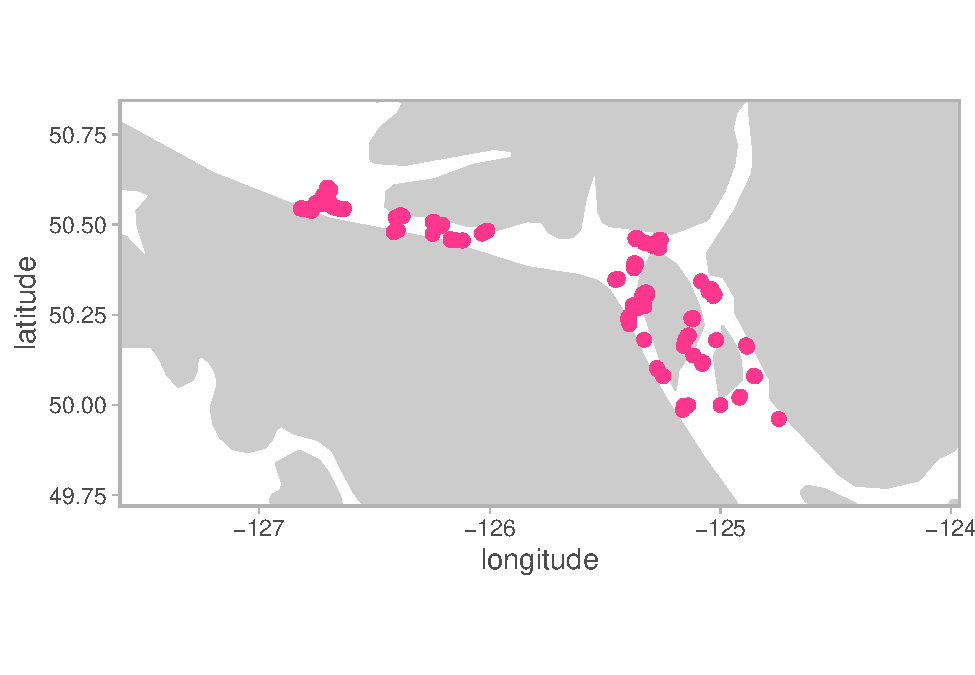
\includegraphics{04-application_files/figure-latex/unnamed-chunk-3-1.pdf}

\begin{Shaded}
\begin{Highlighting}[]
\KeywordTok{ggsave}\NormalTok{(}\KeywordTok{here}\NormalTok{(}\StringTok{"figs"}\NormalTok{, }\StringTok{"basic_map.png"}\NormalTok{))}

\KeywordTok{check_onland}\NormalTok{(DwCA)}
\end{Highlighting}
\end{Shaded}

\begin{verbatim}
## # A tibble: 8,050 x 20
##    occurrenceID basisOfRecord scientificName eventID occurrenceStatus Kingdom
##    <chr>        <chr>         <chr>          <chr>   <chr>            <chr>  
##  1 hakai-jsp-8~ HumanObserva~ Oncorhynchus ~ DE104N1 present          Animal~
##  2 hakai-jsp-8~ HumanObserva~ Oncorhynchus ~ DE104N1 present          Animal~
##  3 hakai-jsp-8~ HumanObserva~ Oncorhynchus ~ DE104N1 present          Animal~
##  4 hakai-jsp-8~ HumanObserva~ Oncorhynchus ~ DE104N1 present          Animal~
##  5 hakai-jsp-8~ HumanObserva~ Oncorhynchus ~ DE104N1 present          Animal~
##  6 hakai-jsp-8~ HumanObserva~ Oncorhynchus ~ DE104N1 present          Animal~
##  7 hakai-jsp-8~ HumanObserva~ Oncorhynchus ~ DE104N1 present          Animal~
##  8 hakai-jsp-8~ HumanObserva~ Oncorhynchus ~ DE104N1 present          Animal~
##  9 hakai-jsp-8~ HumanObserva~ Oncorhynchus ~ DE104N1 present          Animal~
## 10 hakai-jsp-8~ HumanObserva~ Oncorhynchus ~ DE104N1 present          Animal~
## # ... with 8,040 more rows, and 14 more variables: Phylum <chr>, Class <chr>,
## #   Order <chr>, Family <chr>, Genus <chr>, Species <chr>, eventDate <date>,
## #   decimalLatitude <dbl>, decimalLongitude <dbl>, geodeticDatum <chr>,
## #   minimumDepthInMeters <dbl>, maximumDepthInMeters <dbl>,
## #   samplingProtocol <chr>, scientificNameID <dbl>
\end{verbatim}

\begin{Shaded}
\begin{Highlighting}[]
\KeywordTok{check_depth}\NormalTok{(DwCA)}
\end{Highlighting}
\end{Shaded}

\begin{verbatim}
## # A tibble: 262,455 x 20
##    occurrenceID basisOfRecord scientificName eventID occurrenceStatus Kingdom
##    <chr>        <chr>         <chr>          <chr>   <chr>            <chr>  
##  1 hakai-jsp-1  HumanObserva~ Oncorhynchus ~ DE101N1 present          Animal~
##  2 hakai-jsp-2  HumanObserva~ Oncorhynchus ~ DE101N1 present          Animal~
##  3 hakai-jsp-3  HumanObserva~ Oncorhynchus ~ DE101N1 present          Animal~
##  4 hakai-jsp-4  HumanObserva~ Oncorhynchus ~ DE101N1 present          Animal~
##  5 hakai-jsp-5  HumanObserva~ Oncorhynchus ~ DE101N1 present          Animal~
##  6 hakai-jsp-6  HumanObserva~ Oncorhynchus ~ DE101N1 present          Animal~
##  7 hakai-jsp-7  HumanObserva~ Oncorhynchus ~ DE101N1 present          Animal~
##  8 hakai-jsp-8  HumanObserva~ Oncorhynchus ~ DE101N1 present          Animal~
##  9 hakai-jsp-9  HumanObserva~ Oncorhynchus ~ DE101N1 present          Animal~
## 10 hakai-jsp-10 HumanObserva~ Oncorhynchus ~ DE101N1 present          Animal~
## # ... with 262,445 more rows, and 14 more variables: Phylum <chr>, Class <chr>,
## #   Order <chr>, Family <chr>, Genus <chr>, Species <chr>, eventDate <date>,
## #   decimalLatitude <dbl>, decimalLongitude <dbl>, geodeticDatum <chr>,
## #   minimumDepthInMeters <dbl>, maximumDepthInMeters <dbl>,
## #   samplingProtocol <chr>, scientificNameID <dbl>
\end{verbatim}

\begin{Shaded}
\begin{Highlighting}[]
\CommentTok{#(report <- check_outliers_species(DwCA)) # Need to lsid from marinespecies.rg}
\KeywordTok{check_eventdate}\NormalTok{(DwCA)}
\end{Highlighting}
\end{Shaded}

\begin{verbatim}
## # A tibble: 0 x 0
\end{verbatim}

\begin{Shaded}
\begin{Highlighting}[]
\NormalTok{tree <-}\StringTok{ }\KeywordTok{treeStructure}\NormalTok{(event, occurrence)}
\KeywordTok{exportTree}\NormalTok{(tree, }\StringTok{"tree.html"}\NormalTok{)}

\CommentTok{#report(DwCA) # Currently I get warnings on depths. it looks like depths are supposed to be negative? Not according to oceanographers I know. Other points are close to land, need to check closer, but that's expected sampling in the littoral zone.}
\end{Highlighting}
\end{Shaded}

\hypertarget{example-two}{%
\section{Example two}\label{example-two}}

126140

\hypertarget{final-words}{%
\chapter{Final Words}\label{final-words}}

We have finished a nice book.

\bibliography{book.bib,packages.bib}

\end{document}
